% Standalone figure: Morph Edit Distance, BPE vs MorphBPE, all three
% languages. See fertility.tex for the shared styling rationale (mark
% spec, colors -- cyan/purple-blue adapted from the source paper's own
% figure palette -- and single-column sizing).
\documentclass[tikz]{standalone}
\usepackage{times}
\usepackage{pgfplots}
\pgfplotsset{compat=1.18}

\definecolor{seriesBPE}{HTML}{0D9BD0}
\definecolor{seriesMorphBPE}{HTML}{8B5FDB}
\definecolor{gridcolor}{HTML}{E1E0D9}
\definecolor{axiscolor}{HTML}{C3C2B7}
\definecolor{mutedtext}{HTML}{898781}
\definecolor{primaryink}{HTML}{0B0B0B}

\begin{document}
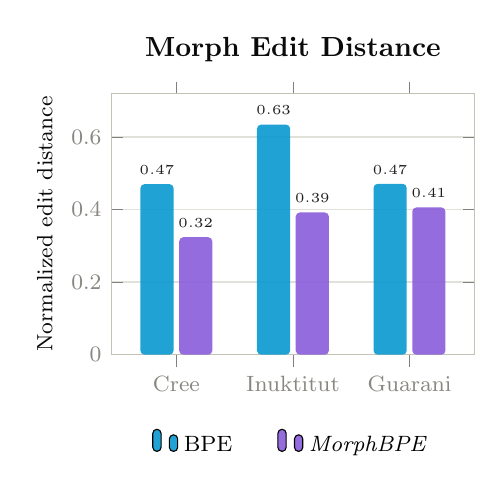
\begin{tikzpicture}
\begin{axis}[
    width=6.2cm, height=4.9cm,
    title={Morph Edit Distance},
    title style={color=primaryink, font=\bfseries\normalsize, yshift=2pt},
    ybar,
    bar width=12pt,
    enlarge x limits=0.28,
    symbolic x coords={Cree,Inuktitut,Guarani},
    xtick=data,
    ymin=0, ymax=0.72,
    ylabel={Normalized edit distance},
    tick label style={color=mutedtext, font=\footnotesize},
    label style={color=primaryink, font=\footnotesize},
    axis line style={axiscolor},
    ymajorgrids=true,
    xmajorgrids=false,
    grid style={gridcolor, line width=0.5pt},
    every axis plot/.append style={draw=none, fill opacity=0.92, rounded corners=1.5pt},
    nodes near coords style={font=\tiny, color=primaryink},
    nodes near coords, every node near coord/.append style={/pgf/number format/.cd, fixed, precision=2},
    legend style={
        at={(0.5,-0.26)}, anchor=north,
        legend columns=-1,
        font=\footnotesize, draw=none, fill=none,
        /tikz/every even column/.append style={column sep=0.5cm},
    },
    legend cell align=left,
]
\addplot[fill=seriesBPE] coordinates {(Cree,0.47010415887966944) (Inuktitut,0.6340606341184748) (Guarani,0.47096764279078007)};
\addlegendentry{BPE}
\addplot[fill=seriesMorphBPE] coordinates {(Cree,0.3237583165134182) (Inuktitut,0.39202809066292077) (Guarani,0.4058784538693111)};
\addlegendentry{\textit{MorphBPE}}
\end{axis}
\end{tikzpicture}
\end{document}
